
\chapter{贪心算法}
今天我们要讲新的内容:贪心算法。

	我们从组合优化的问题开始讲,这个时候我们已经把一个问题给形式化之后,形成了一个组合优化的问题。那接下来我们怎么做呢?我们先看我们能不能正面地解决问题,也就是看这个问题能不能进行规约,及我们能不能把问题变成一个小的问题。如果可以,那我们意识到大概我们能做Divide \&Conquer。或者,整体这一类问题都叫self-reduction。如果在Divide\&Conquer之后,我们还能够再观察到一个结构,也就是上节课讲的Optimal Structure,就意味着我们可以试试动态规划。今天,我们进一步深入,如果这个问题不仅仅可以规约成小的问题,并且它有最优子结构性质,同时它还有第三个性质,贪心选择(Greedy Selection)的性质,那我们就能采取第三类方法:贪心算法。当然,这个贪心算法是一个充满灵感的技巧,以后我们不一定绕这么多,当我们经验丰之后,我们可能一开始就想到这个问题可以用贪心算法来解决。好,今天我们来看看贪心算法。
	
	这堂课我们这么来讲:首先我们从上堂课讲过的最短路径和区间调度(Interval Scheduling)问题开始,这两个问题足够让我们了解贪心算法;接着我们总结一下贪心算法的基本技术;我们还会讲一些其他例子--Huffman编码(Huffman Code),我们都学过,也比较简单,我就跳过去了--只讲讲这个Spanning Tree。为什么要讲它呢?因为我们要讲一点贪心算法的理论基础:拟阵(Matroid),讲拟阵的时候,顺便讲一下最小支撑树;最后我们顺带补充一下为了做最短路径算法而发明的一些数据结构,像:二项堆(Binomial Heap),Fibonacci堆,还有这个我们下次再讲的数据结构:Union-Find。
	
	首先我们做一个声明:这几堂课都是沿着开始上课时我们所讲的解决问题的思路来走。所以首先我们还是要看看一个问题能不能分,这是非常重要的一个性质,也是我们拿到一个问题之后要做的第一个观察。我们一再说如果一个问题能分呢,我们脑子里可以想想看,会有两种分法,拿这个数组为例子:
	这个问题能不能被规约成更小的问题呢?我们从最简单的做起,n个东西不会做,那我们看看一个会不会做,一个会做了,再看看两个会不会做,这是一种规约的策略。
	
	\includegraphics[width=3in]{L5-incremental-dc1.png}
	
	给我n个东西不会做,那我把它一刀砍成两半,看看两个小问题会不会做,非常直白的思路。
	
	\includegraphics[width=3in]{L5-incremental-dc2.png}
	
	好,为了讲贪心算法,我们来看看一个非常实际的问题的两个版本。就拿我们教室来说:可能有很多门课都要来预定这个教室。假如说第i门课程,我们叫它$A_i$,它要从$S_i$这个时候开始上课,到$F_i$结束,那教务处的老师就要利这个时间信息来安排课程。我们已经知道有很多的课程都想来申请我们这间教室,教务处的需求是:能使得越多的学生上课越好。我们举一个例子就清楚了。
	
	 \includegraphics[width=4in] {L7-intervalschedulingexample.eps}
	 
	这是时间轴,每一条黑线代表一门课。我们用W来表示课程有多少学生。我们看看教务处如何安排。我们看看教务可能的安排:
	\begin{enumerate}
		\item 
		选择$\{A_1,A_3,A_5,A_8\}$,这些可的确在时间上不冲突,那能容纳多少学生呢?把这几门课的学生加起来,一共11个学生。
		\item
		选择$\{A_6,A_9\}$,每门课之间也不冲突,总共7个学生可以上课。
	\end{enumerate}
	我想到此,这个问题已经被描叙得很清楚了,就是给我们每门课上课的时间和下课的时间,以及每门课上课的学生,你怎么调度,使得越多的学生上课越好。
	非常清晰哈。
	
	我对这个问题做了一下形式化,但这个形式化大概可以不看,我们只说两个重点吧,其它的我们可以不看。
	\begin{itemize}
		\item
		Compatible:两门课$A_i$和$A_j$compatible,如果它们在时间上没有冲突。
		\item
		我们先假设,所有的课程已经按照它们的结束时间排序,这个要求有点不起眼,但是它很重要,原因我们慢慢再说。
	\end{itemize}
	大家想想,教务处应该怎么处理这九门课?我们做此思维:“还是那个老问题,给我们这么多门课,的确看来,我们搞不定这个事情,那我们看我们能不能把这个问题给变小一点呢?反正九门课我搞不定。能不能把它变小一点?”所以,很多时候,我们碰到的问题的规模很大,一下子可能我们无从下手,我们就想能不能把它变成小的问题,千方百计要琢磨一下这件事情,直到我们发现它的确不好规约,我们再想其他办法,那是啥呢?那等我们下下堂课会讲。现在我们先看,这个问题假如可以被转化成小一点的子问题,那么这个问题的解是啥呢?就是从中间选出来的一个子集。我们把这个求解过程想象成一系列的决策,在每个步骤,我们都要选择一门课。假如我们已经拿到了最优解,我们就问最优解中最后一个决策到底是什么?也就是后一门课$A_n$你是选了呢还是没选?我就看这一件事情!\\
	 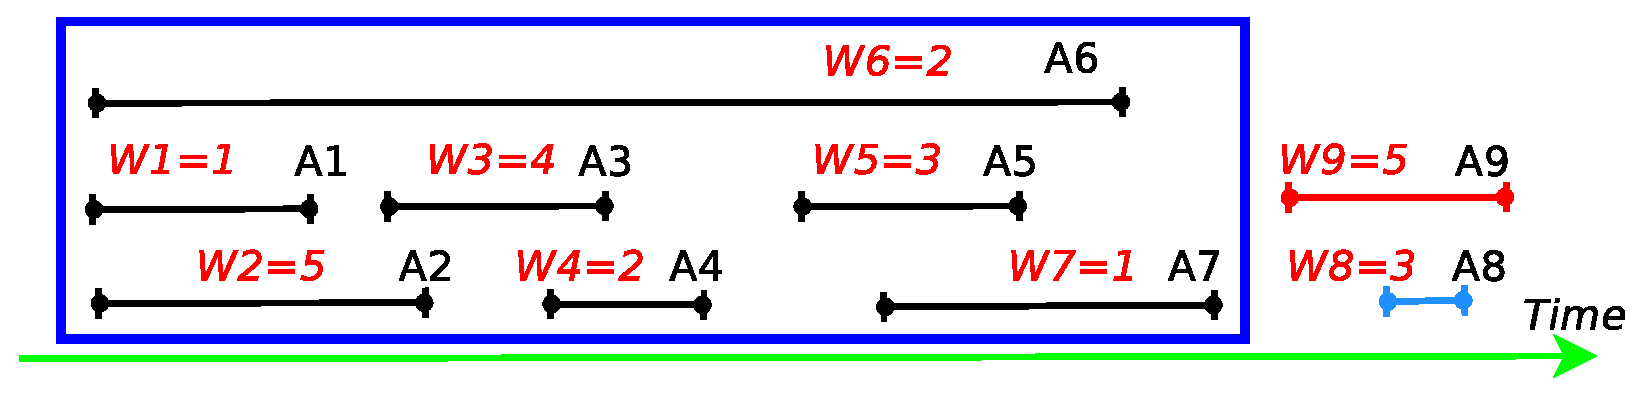
\includegraphics[width=3in] {L7-intervalschedulingexamplek1.eps}\\
	假如说选了这么课$A_9$,那么$A_8$不能选了,因为跟$A_9$时间有冲突,那其它的这些课呢?都跟它没有冲突,那是啥意思呢?就是在你上课之前,我就已经下课了。好,那我剩下的,就是在这蓝框里面所有的课,我们再去选去。对不对?你看,一开始给我们九门课,我们搞不定。选了一门课之后,我们就把问题规约成了一个七门课的问题,我们再去做,因此把问题变小了。那还有一种可能呢?假如说$A_9$这门课我没选,怎么办呢?\\
	 \includegraphics[width=3in] {L7-intervalschedulingexamplek2.eps}\\
	 那意味着,前8门课,甭管跟我打不打架,我都可以来考虑。那剩下的问题就是在前8门课中,我再去选课。那你看:无论是我们选,还是不选$A_9$,我们的确是吧大问题变小了。那变小了这个子问题是什么样子呢?你把这两种情况一总结之后,就可以很清晰地看出这个样子:从$A_1,A_2,…,A_i$当中选择一些课,使能容纳的学生越多越好。
	
	
	现在我们就可以插一句话呢,我们问什么要求这些课要按结束时间排好序呢?假如一开始我们不将它排序,则我们看是否要选一门课,就会有点麻烦。问题变成:
	\[ B(S)=\max\begin{cases}
	B(S-\{a\})\nonumber\\
	B(S-\{a\}-\{\mbox{与}a\mbox{冲突}\})+W_i \nonumber
	\end{cases} \]
	那这两种情况就会很麻烦,你看子问题数目是多少?子问题数目就变成$2^n$了。虽然这个推理是对的,但是就是使得子问题数目比较多。有很多时候,我们要把问题稍微变一下型。
	
	好,我们现在再讲回来。我们观察两种情况之后,把子问题定义成:在前ⅈ门课当中,我们怎么进行选择,使得容纳的学生越多越好,我们把这个最优解记作$opt(i)$,那我们就有这个式子了:
	\[OPT(i) = \max \begin{cases}
	OPT( pre(i) ) + W_i \nonumber\\
	OPT( i-1) \nonumber 
	\end{cases}\]
	其中$pre(i)$表示第$i$门课上课之前已经结束的所有课。大家不妨拿这个公式与前一个公式比较一下,看看差别。都是对的,但是前一个子问题数目太多了,后一个子问题数目是线性的。有了递归表达式之后,我们就能够很容易地写出一个动态规划的算法出来。好,下面我们来看看这个算法的复杂度。
	
	一开始我们对所有的课进行排序,复杂度为$O(n\log(n))$。这个动态规划的时间呢是$O(n)$的,为什么呢?我们看,总共有$n$个子问题,每个子问题只要在两个数中找出最大值,所花的时间是$2n$,加上前面的$O(n\log(n))$,总体的时间还是$O(n\log(n))$的。
	
	现在对这个问题,我们已经做了一个非常好的$O(n\log(n))$的动态规划的算法。下面我们看看这个问题的一点特殊的清晰:假如每门课只有一个学生,我们的目标还是和以前一样,选择一些不冲突的课,容纳的学生越多越好,该怎么办?这相当于把以前的问题变严格了,所以原先的性质还成立,最优子结构的性质还有,不过又多了一个性质,贪心选择的性质。
	
	那什么是贪心选择的性质?对这个问题来说,可以这么陈述:假如$A_1$是下课最早的这门课,那么$A_1$肯定会出现在最优解里。我们来用交换论证(exchange argument)的方法来证明:\\
	 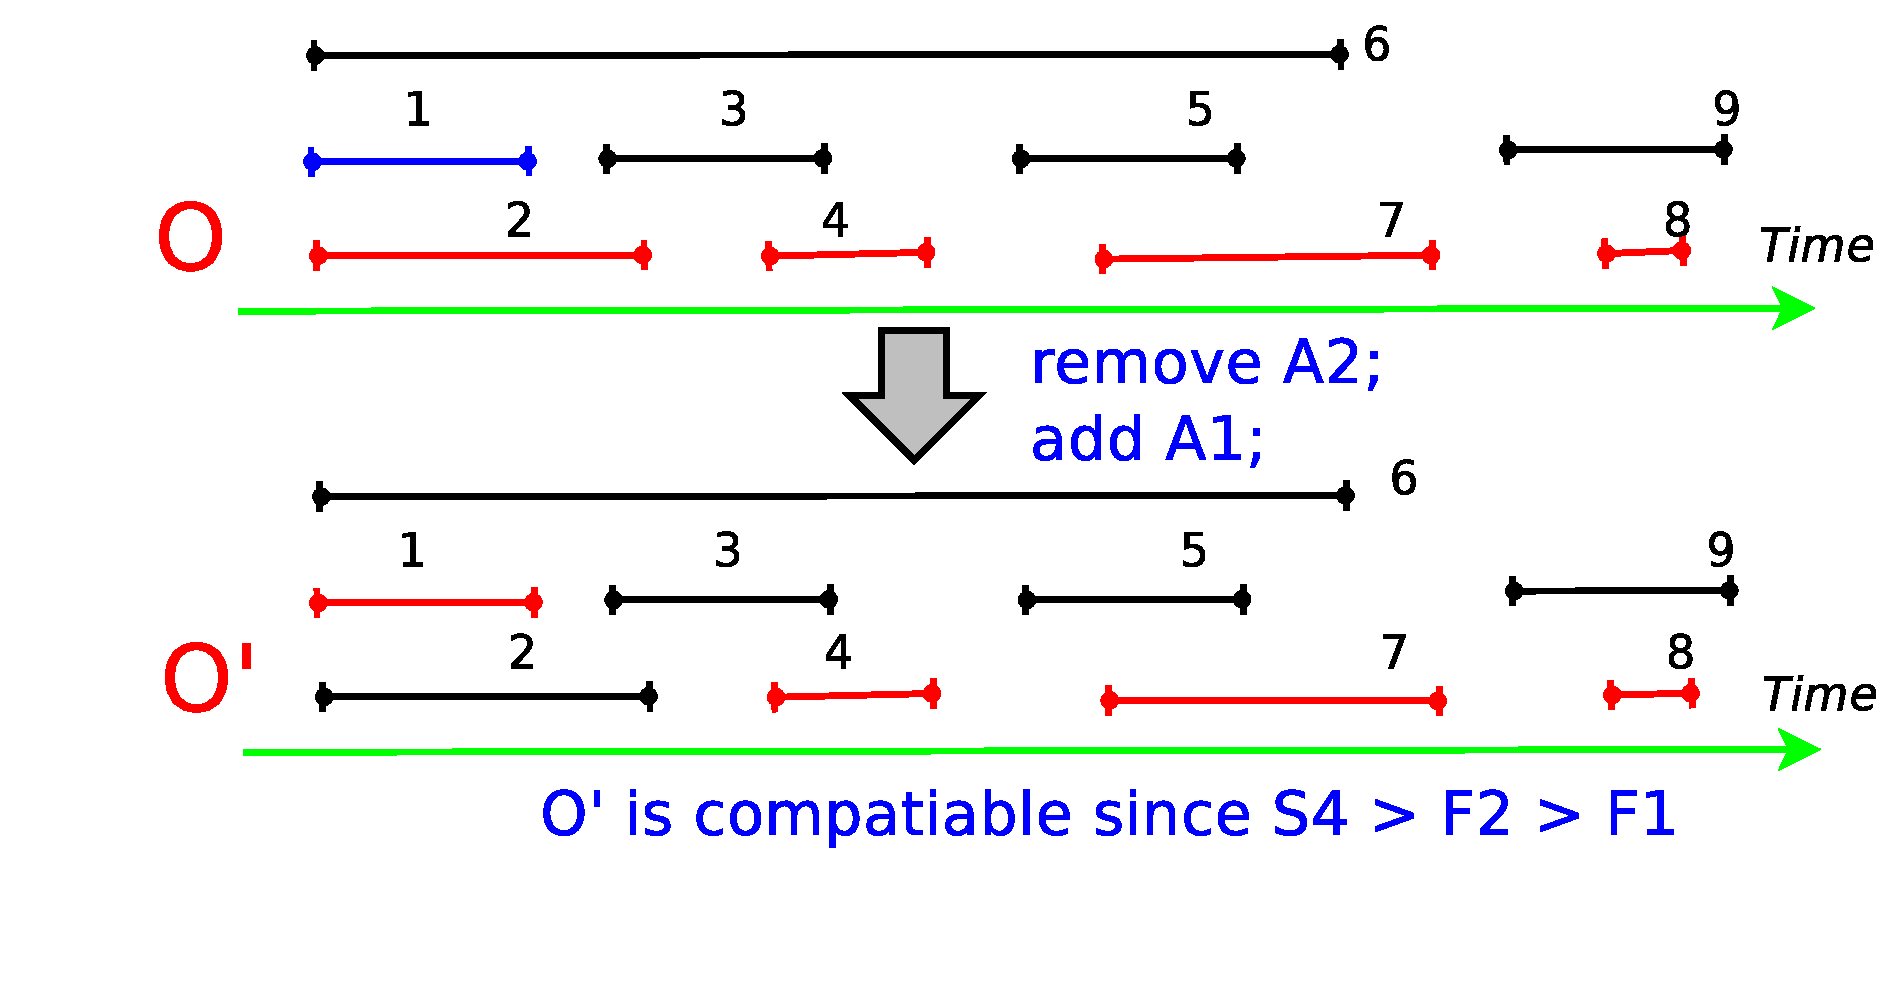
\includegraphics[width=2.9in] {L7-intervalschedulingexampleall1am.eps}\\
	假如有另外的一个最优解$O$,没有选择$A_1$,而是选择了$A_2$。那我们可以自信的说把$A_2$这么课换成$A_1$的话(形成一个新的解$O'$),肯定不会问题,因为$A_1$比$A_2$下课早,所以$A_1$也不会跟$A_2$后面的课冲突。所以$O'$肯定不会比$O$差。有了以上的这些性质,我们就可以将动态规划的算法变成贪心算法。假如所有的课还是按下课时间进行了排序。我们首先选择下课时间最早的这么课$A_1$,接着,我们把所有与$A_1$冲突的课都给去了,然后再不断地往下做。这样我们就把原先的动态规划给简化了。
	\[OPT(i) = \max \begin{cases}
	OPT( pre(i) ) + W_i \nonumber\\
	OPT( i-1) \nonumber 
	\end{cases}\]
	在动态规划里面,我们还要枚举两种case,用来判断是否要选$A_i$,现在我们不用枚举了,只要$A_i$是当下下课最早的课,那我们就直接选。现在这个复杂度还是$O(n\log(n))$,因为最开始我们还是要将课程进行一下排序。现在贪心算法就变得很简单了:
	\begin{itemize}
		\item
		首先,我们选择下课最早的$A_1$,剩下的就只要在蓝色的方框中找最优解就行,就归结成一个更小的子问题了。\\
		 \includegraphics[width=4.1in]{L7-intervalschedulingexamplegreedystep1.eps}
		 \item
		 接下来,就选上一个步骤中蓝色方框里下课最早的课$A_3$,再将蓝色方框缩小。\\
		 \includegraphics[width=4.1in]{L7-intervalschedulingexamplegreedystep2.eps}
		 \item
		 然后,跟之前一样,一步一步构造出一个最优解出来。\\
		 \includegraphics[width=4.1in]{L7-intervalschedulingexamplegreedystep3.eps}\\
		 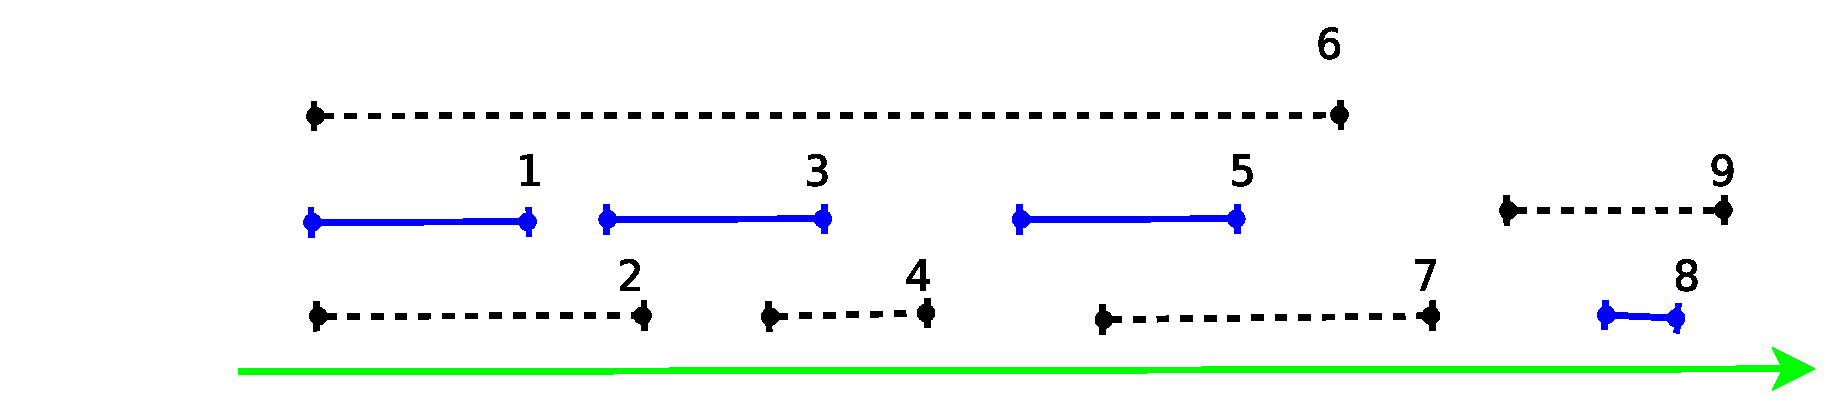
\includegraphics[width=4.1in]{L7-intervalschedulingexamplegreedystep4.eps}
	\end{itemize}
	在动态规划中,最后要的出我们到底选了那些可,还要进行回溯。现在呢,也不用回溯,直接就能够看出了。
	
	现在问一个小的问题,这种贪心的策略在一般的情况下还能够成立吗?不会了。我们看,还是这个一般的情况,及每门课的学生都不一样\\
	\includegraphics[width=4in] {L7-intervalschedulingexample.eps}\\
	按照贪心的办法,我们会选择$ \{ A_1, A_3, A_5, A_8 \} $,总共是11个学生。而最优解是$ \{ A_2, A_4, A_5, A_9 \}$,总共15个学生,只能够通过动态规划算法算出来,贪心算法无能为力。为什么在一般的情况下,贪心算法就不灵光了呢?是因为贪心选择的性质不成立了。所以,大家要注意一下,这两个问题,陈述起来很像,只是这个Weight变了一下,一下就导致算法改变了。
	
	讲到这就能总结一下了,我们看看动态规划和贪心到底有什么异同。首先看相同点:
	\begin{itemize}
		\item
		都是来求解优化的问题
		\item
		都有最优子结构这个性质。不要以为最优子结构是动态规划所独有的,其实不是,贪心算法也要利用到这个性质。
		\item
		最后一点是最深刻的话,“在每一个贪心算法的背后,几乎总会有一个动态规划的算法,算法这个动态规划算法比较笨拙”。这也是为什么诸位本科学算法,通常是先将贪心算法。但我还是倾向于将贪心算法放在动态规划算法之后将,因为前者的确是对后者的一个加强。很多同学都有MIT的那本算法导论,我建议大家看一下贪心算法那章的最后一节(Section),写动态规划和贪心算法之间的关系,写得非常好,是其他书里面所没有的。
	\end{itemize}
	
	我们接着看不同点:
	\begin{itemize}
		\item
		动态规划算法一般需要在所有的决策步(Decision Step)枚举所有的可能性,而且要在所有的子问题被解决之后,才还不能做决定。而贪心根本就没有枚举这一步,而是直接基于局部最优解来做决定,不用考虑这个子问题将来会怎样。(因为无论子问题的结果如何,基于局部最优解所做出的决定总是能够导致全局最优解,这也是贪心选择性质的另外一种表述。)
	\end{itemize}
	
	那到底如何知道该选择贪心算法呢?第一种方法是沿着经典路线:先做Divide\&Conquer,再做动态规划,再做贪心。另外一种:当我们做了很多问题之后,有经验了,我们就试错吧,非常讲究灵感。我们就把求解过程想象成一系列的决策,在每一部,部分解逐步往上涨的时候,尝试不同的贪心选择性质。再次强调,这个需要灵感,在这个过程中,我们可能会犯很多错误。比如说,假如教务处给然我们安排可,我们已经知道,动态规划是可以解决这个问题的,我们再看看贪心算法行不行,而不是沿着经典路线逐步地改善。如何看呢,我们尝试不同的贪心规则:
	\begin{itemize}
		\item
		假如一门课上课越早,就优先安排。\\
		初看这个想法还不错,但一分析,就发现有问题,比如说这样三门课:\\
		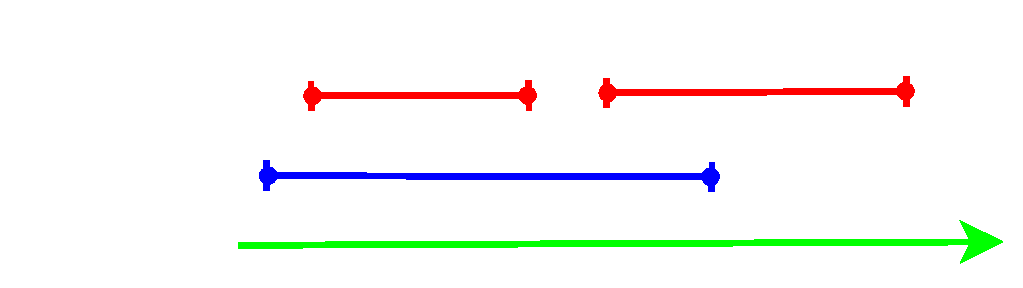
\includegraphics[width=2in]{L7-intervalschedulingexample-error2.eps}\\
		我们看到蓝色的课上课最早,我们就安排它,但实际上是不对的,应该要安排那两门红色的课才对,这样能安排更多。
		\item
		这个就有点tricky了,这个是说如果一门课上课时间短,我们就安排它。\\
		 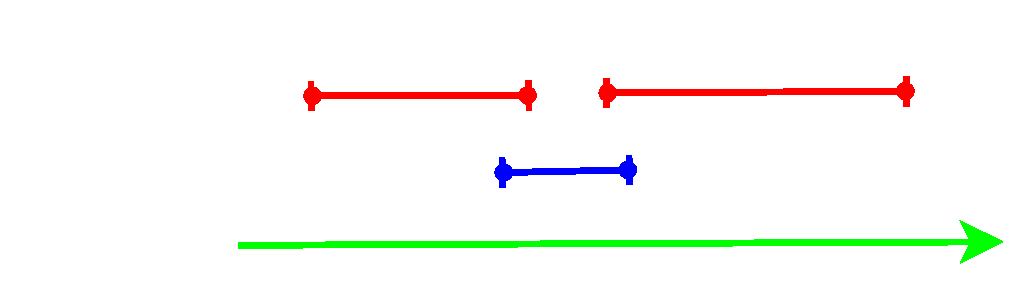
\includegraphics[width=2in]{L7-intervalschedulingexample-error1.eps}\\
		 我们发现这也不行,比如安排了一门蓝色的课后(因为它历时短),两门红色的课就不能选了。
		 \item
		 我们想个更复杂的:如果一门课与其它课冲突很少,就越好。初看这个想法,的确合情合理,大家安排课的时候,的确有可能想到这个方法,可惜还是不对。\\
		 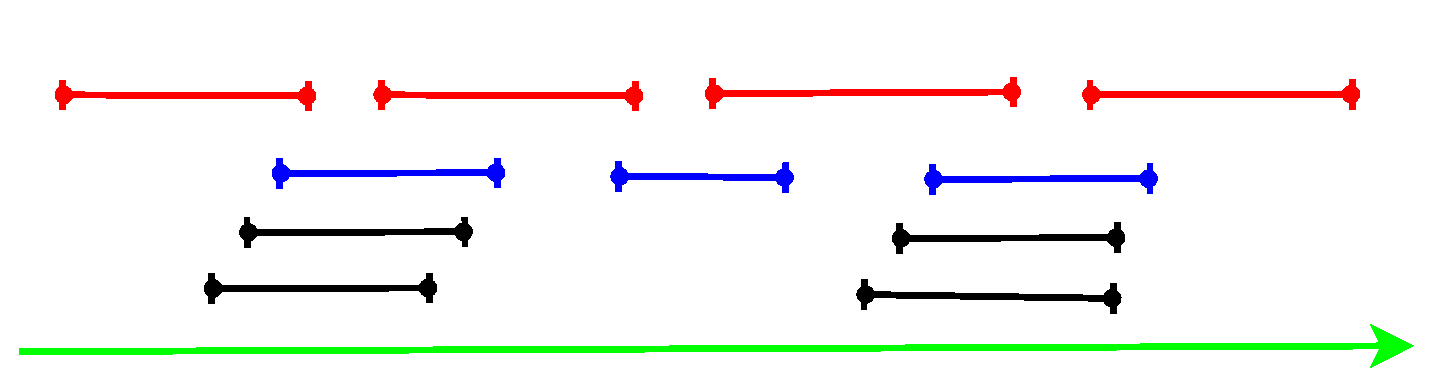
\includegraphics[width=3in]{L7-intervalschedulingexample-error3.eps}\\
		 大家看,中间蓝色那门课只与两门课冲突,根据这个贪心规则,我们首先选它,导致它上面两门红色的课不能选了。于是我们只好选择它旁边两门蓝色的课,这样我们一共选择三门课,但最优解确是选择最上面红色的那四门课。		
	\end{itemize}
	大家看,我们指望我们有灵感,还弄出很复杂的贪心的规则,可最后还是找出了它们的反例。所以,很多时候,我们的灵感真的靠不住,需要我们严谨的验证。这是大家将来写程序会碰到的问题,将来大家碰到一个问题,可能第一想用的办法就是贪心算法,因为它特别的简单,也特别地能体现我们的聪明才智,可是有时候它既是经不起推敲。当然,有时候我们想要找一个反例还挺难的,比如说上面最后那一个例子,我是费老大的劲才找出一个,前面两个到还很easy。
	
	接下来,我们要跟上堂课挂起钩来,我们最短路径问题,很多时候我们从Dijkstra算法开刀,那我们上次课为什么要绕一个弯先讲Bellman-Ford这个动态规划算法呢?就是为了和今天做一些勾连。问题我再简单陈述一下,就是有很多城市,城市之间有不同距离的道路,给了两个城市$s$和$t$,问从$s$到$t$的最短距离是多少?如果没有负圈呢,我们就可以用Bellman-Ford算法,当然,若有负圈,它也能检测出来,所以说它很强大。那如果把条件再加强,不仅没有负圈,而且还没有负边呢?就用不着这个动态规划了,有点费劲,直接做了一个更快的算法,就是Dijkstra贪心算法。
	
	下面我们先回顾一下上节课我们怎么做的这个动态规划算法,然后再看,当改了一下条件,所有边都是正的之后,怎么样进行简化。上堂课我们是这么讲的:我们的解是从$s$到$t$的一条路径,我们还知道$s$到$t$当中,最多只有$n-1$条边,其实这个时候已经把原先的问题变了。原来的问题是这样陈述的:在图$G$当中,我们要找从$s$到$t$的最短路径,记作$d(G,s,t)$。一旦没有负圈的话,我们将问题转换成:求从$s$到$t$当中,最多有$k$条边的路径,记作$d(s,t,k)$。在此,还是再次强调一下,为什么我们要转换问题的描叙呢?因为前者的子问题数目为:$2^n$,而后者是$O(n)$。
	
	好,回顾来,我们把求解过程想象成一系列的决策,每一次决策步决定下一步往哪走。假如我们已经得到一个最优解$O$,我们就观察当中的最后一个决策,是从哪个城市到达$t$,容易得出:凡是能直接到达$t$的点都是有可能的。假如是从$v$到达$t$,剩下的就变成这么一个子问题:如何从$s$到达$v$,最多经过$n-2$条边。所以,我们就可以将子问题的形式写出来了,就是:求从$s$到$v$的距离,最多有$k$步的路径,记作$OPT(v,k)$。那最优子结构的性质就出来了:
	 $OPT(v, k) = \min \begin{cases} 
	 OPT( v, k-1 ) \\
	 {\min_{<u,v>\in E}} \{ OPT( u, k-1) + d_{u, v}  \} \\
	 \end{cases}  $\\
	 上面式子的第一项想要体现的是“至多”,下面一项是枚举所有能到达$v$的$u$,看从哪点过来使得总体的距离最短。这个算法的时间的复杂度是:$O(mn)$,其中$m$,$n$分别是图中边和节点的数目。
	 
	 现在我们跑一下Bellman-Ford这个算法,同时,我们假设每条边都是正的。\\
	 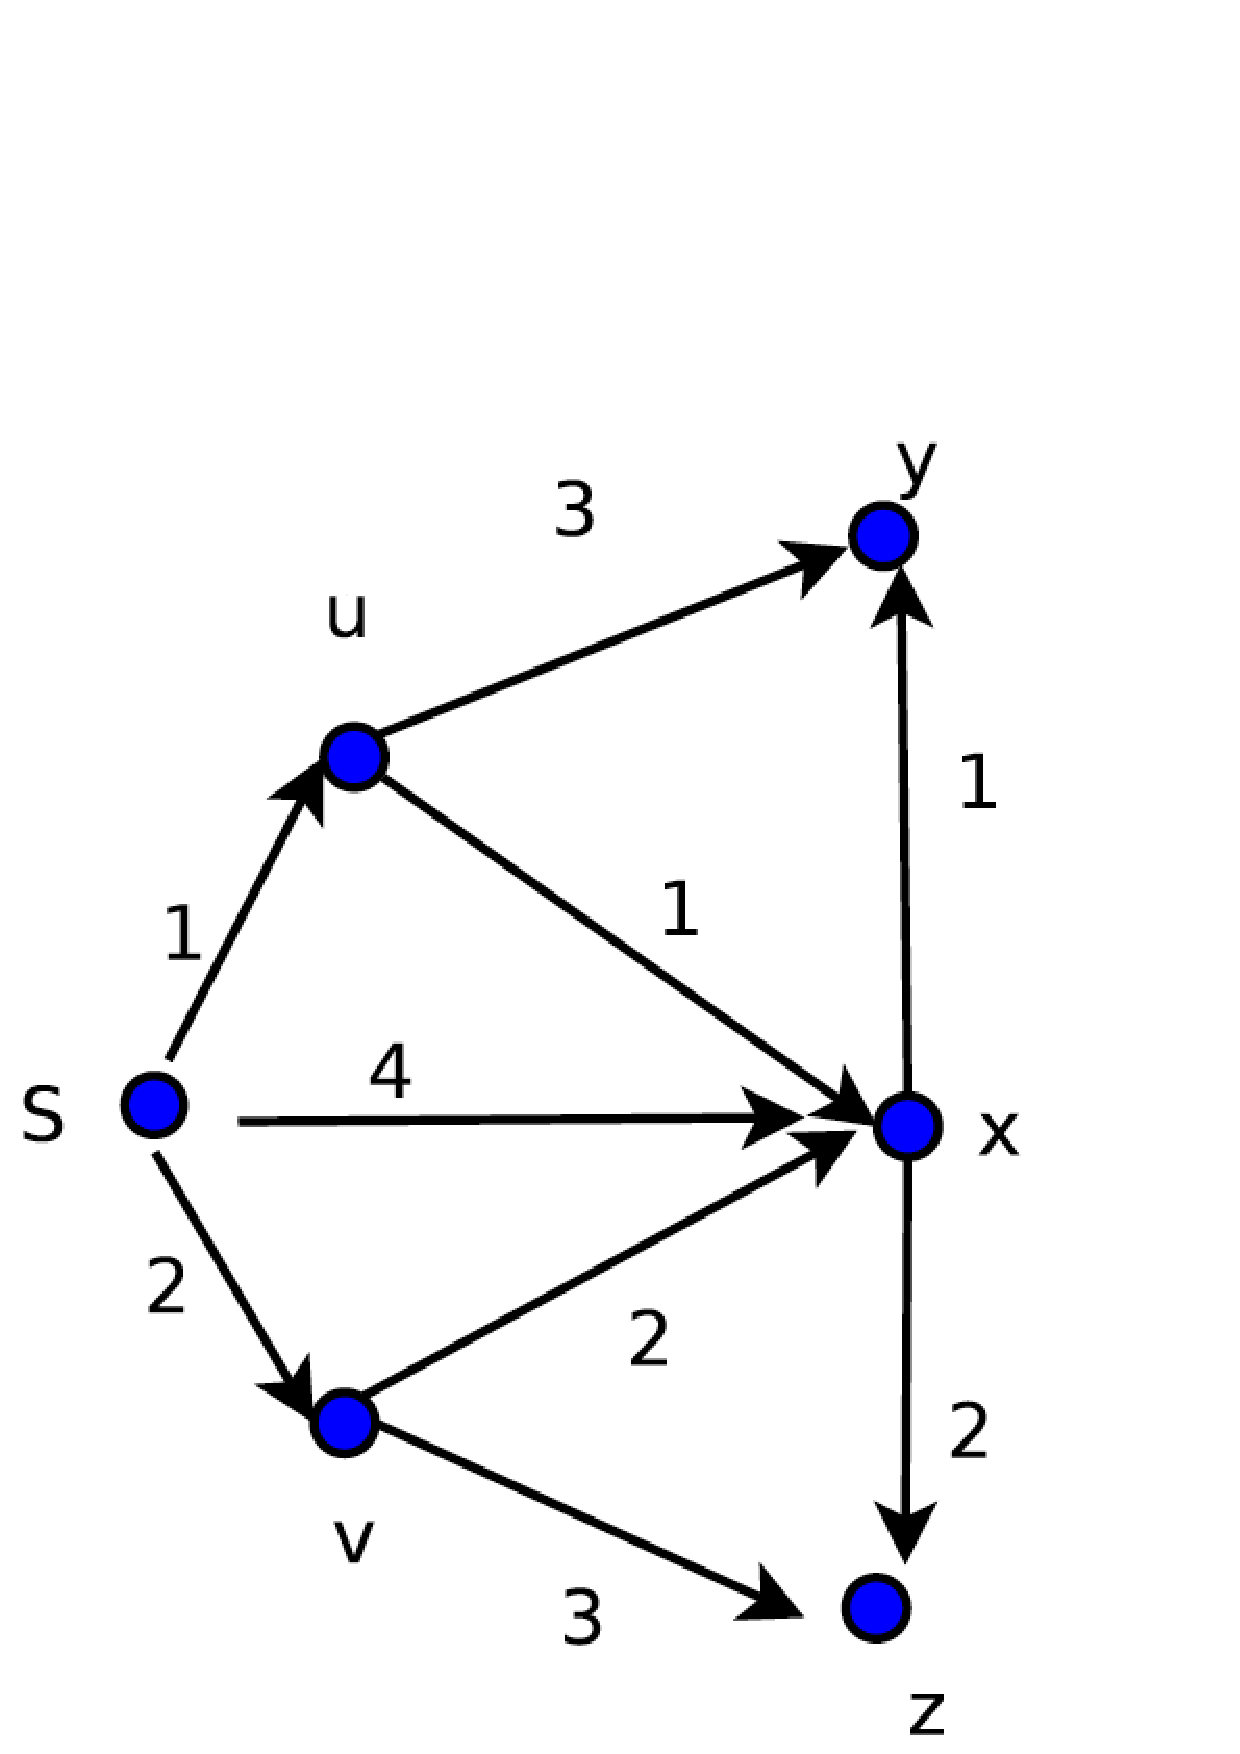
\includegraphics[width=2in]{L7-shortestpathexample.png}
	 \includegraphics[width=2in]{L7-Dijkstraexample.png}\\
	 我们可以得到这样一张表,表的行和列分别是$OPT(v,k)$中的第一,第二个参数。这个表的用处,我们待会再看。
	 
	 我们再看第二个版本,假如说这个边上都是正的,会出什么问题。在算法的第$k$步,我们考察一个特殊的节点$v^\ast$,$v^\ast$是从$s$出发最多经过第$k-1$步能够到达的最近的一个节点。对于$v^\ast$,最优子结构的性质也成立,所以有:\\
	  $OPT(v^\ast, k) = \min \begin{cases} 
	  OPT( v^\ast, k-1 ) \\
	  {\min_{<u,v^\ast>\in E}} \{ OPT( u, k-1) + d_{u, v^\ast}  \} \\
	  \end{cases}  $\\
	 我们仔细看看有什么特殊的地方。光成数学形式上看,我们就可以看出点蹊跷来。我们会发现,上面式子下面的那一部分根本就不用看了,因为下面式子肯定要比上面的大。因为$v^\ast$是是从$s$出发最多经过第$k-1$步能够到达的最近的一个节点,所以$OPT( v^\ast, k-1 ) $肯定要小于${\min_{<u,v^\ast>\in E}} \{ OPT( u, k-1)\} $,我们假设所有边都是正的,所以$d_{u, v^\ast}>0$,所以更加有$OPT( v^\ast, k-1 )>{\min_{<u,v^\ast>\in E}} \{ OPT( u, k-1) + d_{u, v^\ast}  \}$,所以$OPT(v^\ast, k) = OPT( v^\ast, k-1 ) $。这个性质在图中怎么体现呢?大家看图:\\
	 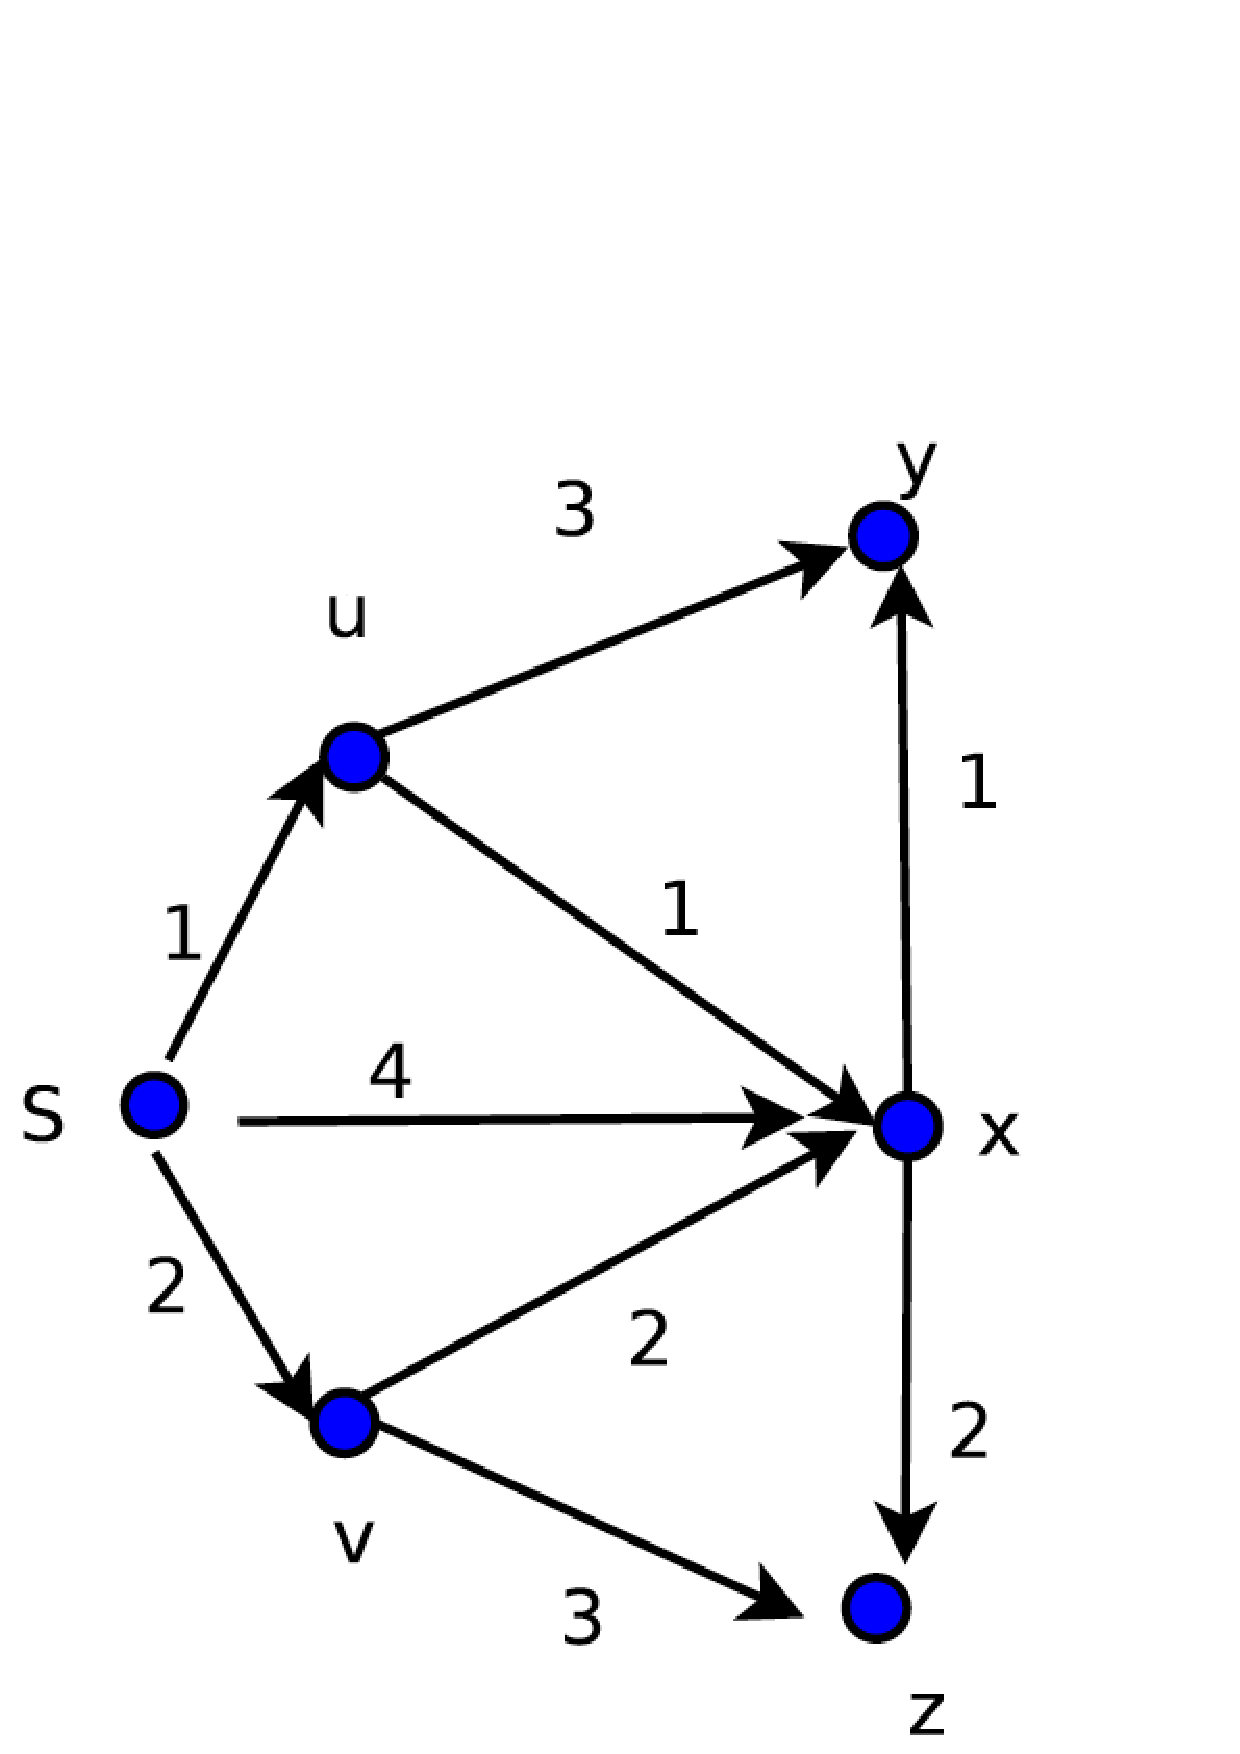
\includegraphics[width=2in]{L7-shortestpathexample.png}
	 \includegraphics[width=2in]{L7-Dijkstraexample.png}\\
	 从列开始看:一旦在一列中间找到最小的值之后(红圈中的值),在看最小值所在行右面的值(绿色方框中的值),永远不变了。最优子结构的性质: $OPT(v, k) = \min \begin{cases} 
	 OPT( v, k-1 ) \\
	 {\min_{<u,v>\in E}} \{ OPT( u, k-1) + d_{u, v}  \} \\
	 \end{cases}  $\\
	 是对任何的节点都成立的。但若我们在所有边都不为负的情况下,对于那些特殊的节点$v^\ast$,最优子结构的性质还用不着,就是$OPT(v^\ast, k) = OPT( v^\ast, k-1 ) $就够了。若是按照Bellman-Ford算法,表中的每一个数值都是要计算的,其实,在所有边都不为负的情况下,所有绿色方框中的值的计算都没有必要,是不用算的。只要计算红色圆圈以及其左边的值就够了,那我们如何来计算这些值呢?我们来看一下一个贪心选择的性质。
	 
	 我们用$S$来表示最短距离已经被确定的点。我们从所有不在$S$中的点中找一个离起始点最近的结点$u^\ast$,所以,从起始点到$u^\ast$的距离可以表示为: $d'(u)=\min_{w\in S}\{d(w)+d(w, u)\}$,并且:最短路径就是:$P=s\rightarrow...\rightarrow w \rightarrow u^*$。
	 
	 下面是算法:
	 {\sc Dijkstra}$(G, s )$
	 \begin{algorithmic}[1]
	 	\STATE $S=\{s\}$; //$S$ denotes the set of explored nodes,
	 	\STATE $d(s)=0$; //$d(u)$ stores an upper bound of the shortest-path weight from $s$ to $u$;
	 	\FORALL{ node $v \neq s$}
	 	\STATE{ $d(v) = +\infty$; } 
	 	\ENDFOR
	 	\WHILE{$S \neq V$}
	 	\FORALL{ node $v \notin S$}
	 	\STATE  $d(v)=\min_{u\in S}\{d(u)+d(u,v)\}$;
	 	\ENDFOR 
	 	\STATE Select the node $v^*$ ($v^* \notin S$) that minimizes $d(v)$;
	 	\STATE $S=S \cup \{v^*\}$;
	 	\ENDWHILE
	 \end{algorithmic}
	 在课程网站上有这个算法的动画演示:Lec7-demo-Dijkstra.pdf。我就即使是不知道Dijkstra当年是怎么想到这个算法的,但是假设我们学了动态规划,学了Bellman-Ford之后,我们也可以写出类似Dijkstra的算法出来,只需要不计算绿色方框中的值就行。
	 
	 这位就是Dijkstra。
	 \includegraphics[width=1.1in]{Dijkstra.jpg}
	 
	 我们再来回顾一下Dijkstra算法和Bellman-Ford算法,我们只是把对边的值的限制稍微改了一下,假如没有负圈,我们有这样一个表达式:
	 $OPT[v, k] = \min \begin{cases}
	 OPT[ v, k-1], \\
	 \min_{<u,v>\in E} \{OPT[u, k-1 ] + d(u,v) \} 
	 \end{cases}$\\
	 如果再加强一下,根本就没有负边,这个约束更强了,导致我们可以用贪心算法。
	 
	 Dijkstra算法的复杂度是$m+n\log n)$,为什么呢?我们将Dijkstra用一个更接近计算机的伪代码描叙出来:
	 {\sc Dijkstra}$( G, s )$
	 \begin{algorithmic}[1]
	 	\STATE $key(s) = 0;$  //$key(u)$ stores an upper bound of the shortest-path weight from $s$ to $u$;
	 	\STATE $PQ.$ {\sc Insert} $(s)$;
	 	\STATE $S=\{ s \}$; // Let $S$ be the set of explored nodes;
	 	\FORALL{ node $v \neq s$ }
	 	\STATE $key(v) = +\infty $
	 	\STATE $PQ.$ {\sc Insert} $(v)$ { \color{red}n times}
	 	\ENDFOR
	 	\WHILE{$ S \neq V $}
	 	\STATE $v=PQ.$ {\sc ExtractMin}$()$;{ \color{red}n times}
	 	\STATE $S=S \cup \{v\}$;
	 	\FOR{ each $w \notin S$ and $<v, w> \in E$}
	 	\IF{ $key(v) + d(v, w) < key(w)$}
	 	\STATE $PQ.${\sc DecreaseKey}($w, key(v) + d(v, w)$); { \color{red}m times}
	 	\ENDIF
	 	\ENDFOR
	 	\ENDWHILE
	 \end{algorithmic}
	 我们定义了一个优先队列(Priority Queue),是什么意思呢?就是里面存了一堆数,我们可以很快找出一个最小来。一开始,把所有的不在$S$中的节点,每个节点都有一个值$+\infty$,我们把它插到优先队列里面去。然后,我们从优先队列里面取一个最小,把最小的数放到$S$当中。接着,对所有墨水没有洇到的那些节点,我们看一下会不会从墨水已经洇得结点当中,重新更新一下路径。所以,一旦能找到一个新的方案,我们更新一下距离。对优先队列,我们有$n$次插入的操作,有$n$次取出最小值的操作,还有$m$次,要把这个值改一下。
	 
	 优先队列我们怎么做呢?有很多种方案。如果大家没有学过优先队列的话,大家也能找出一种方案,本质上即使一堆数之间找最小。\\
  	\begin{tabular}{crrrr}
  		\hline  \hline
  		Operation & Linked  & Binary  & Binomial  & Fibonacci  \\
  		&  list &  heap &  heap & heap \\
  		\hline
  		{\sc MakeHeap} & $ 1 $ &  $1$  & $ 1 $ & $1$  \\ 
  		{\sc Insert} & $ 1 $ &  $\log n$  & $ \log n $ & $1$  \\ 
  		{\sc ExtractMin} & $ n $ &  $\log n$  & $ \log n  $ & $ \log n $  \\ 
  		{\sc DecreaseKey} & $ 1 $ &  $\log n$  & $ \log n $ & $1$  \\ 
  		{\sc Delete} & $ n $ &  $\log n$  & $ \log n $ & $\log n$  \\ 
  		{\sc Union} & $ 1 $ &  $ n $  & $ \log n $ & $1$  \\ 
  		{\sc FindMin} & $ n $ &  $1$  & $ \log n $ & $1$  \\ 
  		\hline 
  		{\sc Dijkstra} & $ O(n^2) $ &  $ O(m \log n) $  & $ O( m \log n ) $ & $ O( m + n \log n) $  \\ 
  		\hline \hline 
  	\end{tabular} \\
  	我们可以写一个数组或链表,讲所有的数存下来。数组和链表,插入一个数只需要$O(1)$的时间,取出最小值得从头到尾都比一遍,需要$O(n)$的时间。现在这个讲的有点快,大家可以先听一下,之后我们会有一个100页的Slide来详细讲。总个Dijkstra算法,需要$O(n*1+m*1+n*n)=O(n^2)$的时间,是所有方法中最老土,最大的。其实,做Dijkstra算法,单是数组不太好,经过一些列的改进,我们最后采用Fibonacci数列,插入只需要$O(1)$的时间,取出最小值要$O(\log n)$,改一下值需要$O(1)$,最终需要$O(m+n\log n)$。就相当于把所有的边枚举一次,把所有的结点排一下序的速度。值得说的是,这个Fibonacci堆就是专门为加快Dijkstra算法专门设计的一种数据结构。
  	
  	好,上节课我们讲到,为了做Dijkstra算法,最老土的办法是数组或链表,但是稍微有点慢。再往下呢,我们可以用一个树结构来存储所有的数,也是本科学到的二叉堆。再往下,我们可以用很多颗树,就是一个森林。再往下,我们可以不仅仅用很多颗树,而且对树的样子不要有太严格的要求,就是Fibonacci堆,做得更快。这里面有很多的设计思想在里面。
  	
  	我们看一下优先队列的核心功能,就是怎么能够存一堆书,以方便我们之后如何能够最快地找最少,而且要考虑到这一堆数还在不断地变。所以,优先队列要支持能这几个功能:
  	\begin{enumerate}
  		\item
  		添加一个数
  		\item
  		在已有的数中找最小
  		\item
  		对数进行修改
  	\end{enumerate}
  	优先队列很有用,很多算法都有用到,比如:
  	\begin{itemize}
  		\item
  		Dijkstra算法
  		\item
  		Prim的最小支撑树
  		\item
  		Huffman编码
  		\item
  		$A^\ast$搜索算法
  		\item
  		HeapSort
  	\end{itemize}
  	反正只要是在一堆数中间找最小,就要用到它。它就干这事。我们下面具体看看Dijkstra算法中是如何用到优先队列的。\\
  	\begin{center}
  		\includegraphics[width=3in]{Dijkstra_demo.png}
  	\end{center}
  	一开始优先队列是这个:$PQ=\{s(0), a(\infty), b(\infty), c(\infty), d(\infty), e(\infty), f(\infty), t(\infty)\}$,除了$s$,其它的数都是正无穷,接着从里面找最小,执行一次,是¥=$s$,接着把与具有当前最小值节点$s$连接的节点的值改一下,比如$a$,原来是正无穷,现在要变成9。
  	\begin{center}
  		\includegraphics[width=3in]{Dijkstra_demo_1.png}
  	\end{center}
  	现在优先队列变成了:$PQ=\{a(9), b(14), c(15), d(\infty), e(\infty), f(\infty), t(\infty) \}$,然后再取出最小值,然后和之前一样,把与具有当前最小值节点$a$连接的节点的值改一下,
  	\begin{center}
  		\includegraphics[width=3in]{Dijkstra_demo_2.png}
  	\end{center}
  	优先队列是:$PQ=\{ b(14), c(15), d(33), e(\infty), f(\infty), t(\infty) \}$。之后再不停的执行这个步骤,每次都是找最小,然后再改一些数。直到优先队列中具有最小值的节点是目标节点$t$。
  	
  	我们怎样来实现这个优先队列呢?先看看最老土的办法,数列。假如我们有一堆数:$[8,1,6,2,4]$,这是一个没有排序的数组。如果新加一个数,我们直接将它放在数组最后面就行了,要花$O(1)$的时间。若找最小呢,那要从头到尾都要找一遍,所以要花$O(n)$的时间。如果我们能够时刻保持数组有序,那求最小就会变得很简单,有序数组为:$[1,2,4,6,8]$只要找第一个数就行,要花$O(1)$的时间,不过插入就麻烦了,比如要插入一个$5$,要从$1$开始比,比到$8$后,在决定放在$8$的前面,可能要与所有的数都比一遍,要花$O(n)$的时间。
  	
  	所以没排序的数列的时间复杂度是这样的:
  	\begin{center}
  		\includegraphics[width=1.5in]{L7-heaptablelinkedlist.png} 
  	\end{center}
  	这有点慢,那怎么办?提出一个新的数据结构:二叉堆,发明人是:R. W. Floyd。它的设计思想:我要放松一下我的要求,但是别放松得太狠。因为有的过强的约束是没有必要的。这也是以下我们要讲的几个数据结构的共同思想。我们的目标是找最小,难道需要所有的数都严格地排序吗?没有必要。但也不能放松得太狠,我们还是要求稍微有点序。
  	\begin{center}
  		\begin{tikzpicture}[scale=1, auto,swap]
  		% Draw a 7,11 network
  		% First we draw the vertices
  		\foreach \pos/\name/\label in {{(0,0)/root/6}, {(-1,-1)/L/10}, {(1,-1)/R/8}, {(-1.5,-2)/LL/12}, {(-.5, -2)/LR/18}, {(0.5, -2)/RL/11}, {(1.5, -2)/RR/25}, {(-1.9, -3)/LLL/21}, {(-1.1, -3)/LLR/17}}
  		\node[middlevertex,draw=black, fill=white!20] (\name) at \pos {\tiny $\label$};
  		
  		% Connect vertices with edges and draw weights
  		\foreach \source/ \dest /\weight in {root/L/{}, root/R/{}, L/LL/{}, L/LR/{}, R/RL/{}, R/RR/{}, LL/LLL/{}, LL/LLR/{}}
  		\path[undirectededge] (\source) -- node[weight] {$\weight$} (\dest);
  		%       \draw[dashed, ->] (0,0) arc  (120:60:2);
  		
  		\foreach \source/ \dest /\weight in {root/L/{},  L/LL/{},  LL/LLR/{}}
  		\path[undirectededge, ultra thick, blue] (\source) -- node[weight] {$\weight$} (\dest);
  		%       \draw[dashed, ->] (0,0) arc  (120:60:2);
  		\end{tikzpicture}
  	\end{center}
  	这个二叉树的特性是:任何一个父亲都比两儿子要小。我们并不要求所有的数都有一个完美的排序,只要求任何一条路径上有序就够了。为什么这样更好呢?因为这是二叉树,任何一条路径只有$\log n$这么高。
  	
  	二叉树有两种实现方式:\\
  	\begin{tikzpicture}[scale=1., auto,swap]
  	% Draw a 7,11 network
  	% First we draw the vertices
  	\foreach \pos/\name/\label in {{(0,0)/root/6}, {(-1,-1)/L/10}, {(1,-1)/R/8}, {(-1.5,-2)/LL/12}, {(-.5, -2)/LR/18}, {(0.5, -2)/RL/11}, {(1.5, -2)/RR/25}, {(-1.9, -3)/LLL/21}}%, {(-1.1, -3)/LLR/17}}
  	\node[middlevertex,draw=black, fill=white!20] (\name) at \pos {\tiny $\label$};
  	
  	\node[above, ultra thick, blue ] at (root.north) {\tiny $1$};
  	\node[above, ultra thick, blue ] at (L.north) {\tiny $2$};
  	\node[above, ultra thick, blue ] at (R.north) {\tiny $3$};
  	\node[above, ultra thick, blue ] at (LL.north) {\tiny $4$};
  	\node[above, ultra thick, blue ] at (LR.north) {\tiny $5$};
  	\node[above, ultra thick, blue ] at (RL.north) {\tiny $6$};
  	\node[above, ultra thick, blue ] at (RR.north) {\tiny $7$}; 
  	\node[above, ultra thick, blue ] at (LLL.north) {\tiny $8$};
  	%    \node[above, ultra thick, blue ] at (LLR.north) {\tiny $9$};
  	
  	
  	% Connect vertices with edges and draw weights
  	\foreach \source/ \dest /\weight in {root/L/{}, root/R/{}, L/LL/{}, L/LR/{}, R/RL/{}, R/RR/{}, LL/LLL/{}}%, LL/LLR/{}}
  	\path[undirectededge] (\source) -- node[weight] {$\weight$} (\dest);
  	%       \draw[dashed, ->] (0,0) arc  (120:60:2);
  	
  	
  	\node[ultra thick, red] at  (2, -1.3) {$\Leftrightarrow$};
  	\def\d{0.5};
  	\def\dy{-1.5};
  	\def\dx{2.5};
  	
  	\foreach \i/\num/\name in { 0/6/s0,1/10/s1,2/8/s2,3/12/s3,4/18/s4, 5/11/s5, 6/25/s6, 7/21/s7, 8/\ /s8, 9/\ /s9, 10/\ /s10} {
  		\draw[  thick ] (\i*\d + \dx,0+\dy) rectangle (\i*\d+\d + \dx, \d + \dy);
  		\node (\name) at (\i*\d+\d/2 + \dx, \d/2 + \dy) {\tiny $\num$};
  	}
  	\node[below, ultra thick, blue ] at (s0.south) {\tiny $1$};
  	\node[below, ultra thick, blue ] at (s1.south) {\tiny $2$};
  	\node[below, ultra thick, blue ] at (s2.south) {\tiny $3$};
  	\node[below, ultra thick, blue ] at (s3.south) {\tiny $4$};
  	\node[below, ultra thick, blue ] at (s4.south) {\tiny $5$};
  	\node[below, ultra thick, blue ] at (s5.south) {\tiny $6$};
  	\node[below, ultra thick, blue ] at (s6.south) {\tiny $7$};
  	\node[below, ultra thick, blue ] at (s7.south) {\tiny $8$};
  	\node[below, ultra thick, blue ] at (s8.south) {\tiny $9$};
  	\node[below, ultra thick, blue ] at (s9.south) {\tiny $10$};
  	\node[below, ultra thick, blue ] at (s10.south) {\tiny $11$};
  	
  	\end{tikzpicture}\\
  	第一种方法是老老实实的存下两个子节点的指针,还可以干脆将其弄成一个数组就行,这样,第$k$个节点的父亲就是第$k/2$个节点。假如我们采取第二种方式。这样,我们就只要这个数组中部分有序就够了,相当于放松了一下要求。我们还要对二项堆进行一些基本操作,当HeapOrder(父节点要比其子节点小)被违反了之后,则通过交换节点的方法,讲HeapOrder保持下去。\\
	\begin{tikzpicture}[auto,swap]
	
	\foreach \pos/\name/\label in {{(0,0)/root/6}, {(-1,-1)/L/10}, {(1,-1)/R/8}, {(-1.5,-2)/LL/18}, {(0.5, -2)/RL/11}, {(1.5, -2)/RR/25}, {(-1.9, -3)/LLL/21}}%, {(-1.1, -3)/LLR/7}}
	\node[middlevertex,draw=black, fill=white!20] (\name) at \pos {\tiny $\label$};
	
	\foreach \pos/\name/\label in {{(-1.1, -3)/LLR/27}}
	\node[middlevertex,draw=black, fill=white!20] (\name) at \pos {\tiny $\label$};
	
	\foreach \pos/\name/\label in { {(-1,-1)/L/15}}
	\node[middlevertex,draw=black, fill=green!20] (\name) at \pos {\tiny $\label$};
	
	\foreach \pos/\name/\label in { {(-.5, -2)/LR/13}}
	\node[middlevertex,draw=black, fill=red!20] (\name) at \pos {\tiny $\label$};
	
	\foreach \source/ \dest /\weight in {root/L/{}, root/R/{}, L/LL/{}, L/LR/{}, R/RL/{}, R/RR/{}, LL/LLL/{},  LL/LLR/{}}
	\path[undirectededge] (\source) -- node[weight] {$\weight$} (\dest);
	\end{tikzpicture}
	\begin{tikzpicture}[ auto,swap]
	
	\foreach \pos/\name/\label in {{(0,0)/root/6}, {(1,-1)/R/8},   {(-1.5,-2)/LL/18}, {(0.5, -2)/RL/11},  {(1.5, -2)/RR/25}, {(-1.9, -3)/LLL/21}, {(-1.1, -3)/LLR/27}}%, {(-1.1, -3)/LLR/7}}
	\node[middlevertex,draw=black, fill=white!20] (\name) at \pos {\tiny $\label$};
	
	\foreach \pos/\name/\label in {{(-1,-1)/L/13}}
	\node[middlevertex,draw=black, fill=red!20] (\name) at \pos {\tiny $\label$};
	
	\foreach \pos/\name/\label in {{(-.5, -2)/LR/15}}
	\node[middlevertex,draw=black, fill=green!20] (\name) at \pos {\tiny $\label$};    
	
	\foreach \source/ \dest /\weight in {root/L/{}, root/R/{}, L/LL/{}, L/LR/{}, R/RL/{}, R/RR/{}, LL/LLL/{},  LL/LLR/{}}
	\path[undirectededge] (\source) -- node[weight] {$\weight$} (\dest);
	
	\foreach \source/ \dest /\weight in {L/LL/{},  LL/LLR/{}}
	\path[undirectededge] (\source) -- node[weight] {$\weight$} (\dest);
	
	\end{tikzpicture}\\
	比如上面这个图,左边的HeapOrder被打乱了,于是我们交换值为15与值为13的节点的位置。若用二叉堆表示了一堆数之后,则求最小的问题就变得很简单了,因为父亲的值总比儿子的小,那么求最小就只要看根节点就好了。当我们先插入一个数时,先把它放到树的最下面,这可能会破坏HeapOrder规则,但我们可以通过一系列的交换来重新维护规则。该值也是同样的道理。
	
	假如我们在Dijkstra算法中用到了二项堆,那算法的时间复杂度是多少呢?算法中最多只有$m$项插入,换值和取出最小值操作,每次操作最多花$\log n$时间,所以总体的复杂度是$O(m\log n)$。
 	
  	我们看,二叉堆相比用单纯的数组或是链表,它放松了一些,不要要求所有的数都有序。但是用二叉堆,两个堆的合并要花$O(n)$的时间。\\
  	\begin{tikzpicture}[scale=0.9, auto,swap]
  	
  	\foreach \pos/\name/\label in {{(0,0)/root/21}, {(-1,-1)/L/25}, {(1,-1)/R/27}, {(-1.5,-2)/LL/29}}
  	\node[middlevertex,draw=black, fill=white!20] (\name) at \pos {\tiny $\label$};
  	\foreach \source/ \dest /\weight in {root/L/{}, root/R/{}, L/LL/{}}
  	\path[undirectededge] (\source) -- node[weight] {$\weight$} (\dest);
  	
  	\node[ultra thick, above, blue] at (root.north)  {$H_1$}; 
  	
  	\foreach \pos/\name/\label in {{(4+0,0)/root/6}, {(4-1,-1)/L/8}, {(4+1,-1)/R/11}}
  	\node[middlevertex,draw=black, fill=white!20] (\name) at \pos {\tiny $\label$};
  	\foreach \source/ \dest /\weight in {root/L/{}, root/R/{}}
  	\path[undirectededge] (\source) -- node[weight] {$\weight$} (\dest);
  	\node[ultra thick, above, blue] at (root.north)  {$H_2$}; 
  	\end{tikzpicture}\\
  	比如上面是两个二叉堆,我们想把它们合成一个。一种方法是把一个中的每一个数一个个地插入到另外一个二叉堆中,这是可以得,但是很慢。另外一种呢,把所有的数都拿过来,放在一起,然后重新建堆,这个要花$O(n)$的时间。那我们想有没有更快的方法呢?我们再想想我们一定需要将两个堆合并成一个吗,我们可不可以用多颗树来装下所有树呢?这就是下面我们要讲的二项树(Binomial Heap)的思想。这就是更进一步的放松了,我们之前要求要用一棵树来表示所有的树,现在我们放松到可以用多颗树来表示。这样,合并操作相当于就只要花$O(n)$的时间。但是我们还要记得一点,我们不能过分放松了,因为之后我们还要在所有的数中间找最小呢。用多颗树表示的话,我们如何在所有数之间找最小呢?由于每棵树的最小值都是它的根,那我们只要在所有树的根之间找最小就行。这种方法最极端的例子是什么?那就是每个数字单独形成一个数,这样就相当于回到了一开始用数组的方法,我们需要在所有数当中取出最小值。这有很麻烦。所以二项树思想最光辉的思想就在这,可以允许用多棵树来表示,但不要有太多,太多了又麻烦了。那怎么做到这一点呢?于是我们发现树太多了,我们就将他们合并一下。具体方法叫做consolidating:\\
  	\begin{tikzpicture}[scale=0.9, auto,swap]
  	
  	\def\dx{0};
  	\def\dy{1.5};
  	\foreach \pos/\name/\label in {{(0 +\dx,0 +\dy)/root/6}, {(1.5 + \dx, 0 + \dy)/L/11}} 
  	\node[middlevertex,draw=black, fill=white!20] (\name) at \pos {\tiny $\label$};
  	
  	
  	
  	\draw[->, line width=2pt, blue] (2, 2-0.5) -- node[above]{$link$} (3, 2-0.5); 
  	\def\dx{3.5};
  	\def\dy{2};
  	\foreach \pos/\name/\label in {{(0 +\dx,0 +\dy)/root/6}, {(0 + \dx, -1 + \dy)/L/11}} 
  	\node[middlevertex,draw=black, fill=white!20] (\name) at \pos {\tiny $\label$};
  	\foreach \source/ \dest /\weight in {root/L/{}}
  	\path[undirectededge] (\source) -- node[weight] {$\weight$} (\dest);
  	
  	
  	
  	\def\dx{0};
  	\def\dy{0};
  	\foreach \pos/\name/\label in {{(0 +\dx,0 +\dy)/root/6}, {(0 + \dx, -1 + \dy)/L/11}} 
  	\node[middlevertex,draw=black, fill=white!20] (\name) at \pos {\tiny $\label$};
  	\foreach \source/ \dest /\weight in {root/L/{}}
  	\path[undirectededge] (\source) -- node[weight] {$\weight$} (\dest);
  	
  	
  	\def\dx{1.5};
  	\def\dy{0};
  	\foreach \pos/\name/\label in {{(0 +\dx,0 +\dy)/root/8}, {(0 + \dx, -1 + \dy)/L/9}} 
  	\node[middlevertex,draw=black, fill=white!20] (\name) at \pos {\tiny $\label$};
  	\foreach \source/ \dest /\weight in {root/L/{}}
  	\path[undirectededge] (\source) -- node[weight] {$\weight$} (\dest);
  	
  	\draw[->, line width=2pt, blue] (2, -0.5) -- node[above]{$link$} (3, -0.5); 
  	
  	
  	\def\dx{3.5};
  	\def\dy{0};
  	\foreach \pos/\name/\label in {{(0 +\dx,0 +\dy)/root/6}, {(0 + \dx, -1 + \dy)/L/11}} 
  	\node[middlevertex,draw=black, fill=white!20] (\name) at \pos {\tiny $\label$};
  	\foreach \source/ \dest /\weight in {root/L/{}}
  	\path[undirectededge] (\source) -- node[weight] {$\weight$} (\dest);
  	
  	
  	\def\dx{4.5};
  	\def\dy{-1};
  	\foreach \pos/\name/\label in {{(0 +\dx,0 +\dy)/R/8}, {(0 + \dx, -1 + \dy)/RL/9}} 
  	\node[middlevertex,draw=black, fill=white!20] (\name) at \pos {\tiny $\label$};
  	\foreach \source/ \dest /\weight in {R/RL/{}, root/R/{}}
  	\path[undirectededge] (\source) -- node[weight] {$\weight$} (\dest);
  	
  	
  	\end{tikzpicture}\\
  	那具体怎么合并呢?我们只要比较一下两颗树根的大小,把大的那棵树接在小的那一颗树的根节点的下面,以保持HeapOrder。我们下面给出二项树一个严格的定义,这是一个递归定义的:
  	\begin{itemize}
  		\item
  		单个节点可以叫做一个二项树。
  		\item
  		一个二项树一定由两个相同大小的二项树按照规则(比较一下两颗树根的大小,把大的那棵树接在小的那一颗树的根节点的下面)组成。
  	\end{itemize}
  	比如,下面几个图都是二项树:\\
  	\begin{center}
  		\begin{tikzpicture}[scale=1., auto,swap]
  		
  		\def\dx{0};
  		\def\dy{0}; 
  		\def\u{0.8};
  		
  		\foreach \x/\y/\name/\label in { 0/0/root/6, 0/-1/L11/8, 1/-1/L12/9, 1/-2/L21/10}
  		\node[smallvertex,draw=black, fill=white!20] (\name) at (\x*\u+\dx, \y + \dy) {\tiny $\label$};
  		
  		
  		
  		\foreach \source/ \dest /\weight in {root/L11/{}, root/L12/{}}
  		\path[undirectededge] (\source) -- node[weight] {$\weight$} (\dest);
  		
  		
  		
  		\foreach \source/ \dest /\weight in {L12/L21/{}}
  		\path[undirectededge] (\source) -- node[weight] {$\weight$} (\dest);
  		
  		
  		
  		\node[above, blue, ultra thick] at (root.north) {$B_2$};
  		
  		
  		\def\dx{2};
  		\def\dy{0}; 
  		\def\u{0.8};
  		
  		\foreach \x/\y/\name/\label in { 0/0/root/6, 0/-1/L11/8, 1/-1/L12/9, 2/-1/L13/7} 
  		\node[smallvertex,draw=black, fill=white!20] (\name) at (\x*\u+\dx, \y + \dy) {\tiny $\label$};
  		
  		\foreach \x/\y/\name/\label in {1/-2/L21/10, 2/-2/L22/11/, 3/-2/L23/12}
  		\node[smallvertex,draw=black, fill=white!20] (\name) at (\x*\u+\dx, \y + \dy) {\tiny $\label$};
  		
  		\foreach \x/\y/\name/\label in {3/-3/L31/14}
  		\node[smallvertex,draw=black, fill=white!20] (\name) at (\x*\u+\dx, \y + \dy) {\tiny $\label$};
  		
  		
  		\foreach \source/ \dest /\weight in {root/L11/{}, root/L12/{}, root/L13/{}}
  		\path[undirectededge] (\source) -- node[weight] {$\weight$} (\dest);
  		
  		\foreach \source/ \dest /\weight in {L12/L21/{}, L13/L22/{}, L13/L23/{}, L23/L31/{}}
  		\path[undirectededge] (\source) -- node[weight] {$\weight$} (\dest);
  		
  		
  		\node[above, blue, ultra thick] at (root.north) {$B_3$};
  		
  		
  		\end{tikzpicture}
  			
		\begin{tikzpicture}[scale=1., auto,swap]
		
		\def\dx{0};
		\def\dy{0}; 
		\def\u{0.8};
		
		\foreach \x/\y/\name/\label in { 0/0/root/0, 0/-1/L11/8, 1/-1/L12/9, 2/-1/L13/7, 4/-1/L14/5} 
		\node[smallvertex,draw=black, fill=white!20] (\name) at (\x*\u+\dx, \y + \dy) {\tiny $\label$};
		
		\foreach \x/\y/\name/\label in {1/-2/L21/10, 2/-2/L22/11/, 3/-2/L23/12, 4/-2/L24/11, 5/-2/L25/12, 6/-2/L26/13}
		\node[smallvertex,draw=black, fill=white!20] (\name) at (\x*\u+\dx, \y + \dy) {\tiny $\label$};
		
		\foreach \x/\y/\name/\label in {3/-3/L31/14, 5/-3/L32/14, 6/-3/L33/15, 7/-3/L34/16}
		\node[smallvertex,draw=black, fill=white!20] (\name) at (\x*\u+\dx, \y + \dy) {\tiny $\label$};
		
		
		\foreach \x/\y/\name/\label in {7/-4/L41/17}
		\node[smallvertex,draw=black, fill=white!20] (\name) at (\x*\u+\dx, \y + \dy) {\tiny $\label$};
		
		
		\foreach \source/ \dest /\weight in {root/L11/{}, root/L12/{}, root/L13/{}, root/L14/{}}
		\path[undirectededge] (\source) -- node[weight] {$\weight$} (\dest);
		
		\foreach \source/ \dest /\weight in {L12/L21/{}, L13/L22/{}, L13/L23/{}, L14/L24/{}, L14/L25/{}, L14/L26/{}, L23/L31/{}, L25/L32/{}, L26/L33/{}, L26/L34/{}, L34/L41/{}}
		\path[undirectededge] (\source) -- node[weight] {$\weight$} (\dest);
		
		
		\node[above, blue, ultra thick] at (root.north) {$B_4$};
		
		
		
		\end{tikzpicture}
  	\end{center}
  	
  	我们看看这个数有什么特点:任何一个树都不是特别平衡,但每个数的节点都有这样一些性质:
  	\begin{enumerate}
  		\item $|B_k|=2^k$; 
  		\item $height(B_k)=k$; 
  		\item $degree(B_k) = k$; 
  		\item 第$i$个儿子有 $i-1$个儿子; 
  	\end{enumerate}
  	一个二项堆其实不是一棵树了,它是很多棵树:\\
  	\begin{tikzpicture}[scale=1., auto,swap]
  	
  	
  	
  	\draw[thick, dashed, blue] (0,0) -- (4,0);
  	%B0
  	\def\dx{0};
  	\def\dy{0}; 
  	\def\u{0.8};
  	
  	\foreach \x/\y/\name/\label in { 0/0/root/3}
  	\node[smallvertex,draw=black, fill=white!20] (\name) at (\x*\u+\dx, \y + \dy) {\tiny $\label$};
  	
  	\node[ultra thick, blue, above] at (root.north) {$B_0$};  
  	
  	%B1
  	\def\dx{1};
  	\def\dy{0}; 
  	\def\u{0.8};
  	
  	\foreach \x/\y/\name/\label in { 0/0/root/4, 0/-1/L11/8}
  	\node[smallvertex,draw=black, fill=white!20] (\name) at (\x*\u+\dx, \y + \dy) {\tiny $\label$};
  	
  	
  	
  	\foreach \source/ \dest /\weight in {root/L11/{}}
  	\path[undirectededge] (\source) -- node[weight] {$\weight$} (\dest);
  	
  	
  	\node[ultra thick, blue, above] at (root.north) {$B_1$};  
  	
  	%B2
  	\def\dx{2};
  	\def\dy{0}; 
  	\def\u{0.8};
  	
  	\foreach \x/\y/\name/\label in { 0/0/root/5, 0/-1/L11/8, 1/-1/L12/9, 1/-2/L21/10}
  	\node[smallvertex,draw=black, fill=white!20] (\name) at (\x*\u+\dx, \y + \dy) {\tiny $\label$};
  	
  	
  	
  	\foreach \source/ \dest /\weight in {root/L11/{}, root/L12/{}}
  	\path[undirectededge] (\source) -- node[weight] {$\weight$} (\dest);
  	
  	
  	
  	\foreach \source/ \dest /\weight in {L12/L21/{}}
  	\path[undirectededge] (\source) -- node[weight] {$\weight$} (\dest);
  	
  	\node[ultra thick, blue, above] at (root.north) {$B_2$};  
  	
  	%B3
  	
  	\def\dx{4};
  	\def\dy{0}; 
  	\def\u{0.8};
  	
  	\foreach \x/\y/\name/\label in { 0/0/root/6, 0/-1/L11/8, 1/-1/L12/9, 2/-1/L13/7} 
  	\node[smallvertex,draw=black, fill=white!20] (\name) at (\x*\u+\dx, \y + \dy) {\tiny $\label$};
  	
  	\foreach \x/\y/\name/\label in {1/-2/L21/10, 2/-2/L22/11/, 3/-2/L23/12}
  	\node[smallvertex,draw=black, fill=white!20] (\name) at (\x*\u+\dx, \y + \dy) {\tiny $\label$};
  	
  	\foreach \x/\y/\name/\label in {3/-3/L31/14}
  	\node[smallvertex,draw=black, fill=white!20] (\name) at (\x*\u+\dx, \y + \dy) {\tiny $\label$};
  	
  	
  	\foreach \source/ \dest /\weight in {root/L11/{}, root/L12/{}, root/L13/{}}
  	\path[undirectededge] (\source) -- node[weight] {$\weight$} (\dest);
  	
  	\foreach \source/ \dest /\weight in {L12/L21/{}, L13/L22/{}, L13/L23/{}, L23/L31/{}}
  	\path[undirectededge] (\source) -- node[weight] {$\weight$} (\dest);
  	
  	\node[ultra thick, blue, above] at (root.north) {$B_3$};  
  	
  	
  	
  	\end{tikzpicture}
   每棵树是同样满足一定的排序的。而且每一个$k$级树最多只有一颗,因为若有多颗,我们需要将它们合并。所以要容纳$n$棵树,整个森林中最多只有 $\lfloor \log_2 n \rfloor + 1 $棵树,并且最高的那棵树的高度是 $\lfloor \log_2 n \rfloor$。所以在所有数中间找最小,我们只需要在树的根节点中间找,只要花$O(\log n)$的时间。接下来我们看看讲两组树合并需要花多少时间?\\
   \begin{tikzpicture}[scale=1., auto,swap]
   
   
   
   \draw[thick, dashed, blue] (0,0) -- (2,0);
   
   \draw[thick, dashed, blue] (4,0) -- (6,0);
   
   \node[ultra thick, red] at (3.5, -0.5) {\Large $+$};
   %B0
   \def\dx{0};
   \def\dy{0}; 
   \def\u{0.8};
   
   \foreach \x/\y/\name/\label in { 0/0/root/3}
   \node[smallvertex,draw=black, fill=white!20] (\name) at (\x*\u+\dx, \y + \dy) {\tiny $\label$};
   
   
   \node[ultra thick, blue, above] at (root.north) {$B_0$};  
   
   %B1
   \def\dx{4};
   \def\dy{0}; 
   \def\u{0.8};
   
   \foreach \x/\y/\name/\label in { 0/0/root/4, 0/-1/L11/8}
   \node[smallvertex,draw=black, fill=white!20] (\name) at (\x*\u+\dx, \y + \dy) {\tiny $\label$};
   
   
   
   \foreach \source/ \dest /\weight in {root/L11/{}}
   \path[undirectededge] (\source) -- node[weight] {$\weight$} (\dest);
   
   
   \node[ultra thick, blue, above] at (root.north) {$B_1$};  
   
   %B2
   \def\dx{2};
   \def\dy{0}; 
   \def\u{0.8};
   
   \foreach \x/\y/\name/\label in { 0/0/root/5, 0/-1/L11/8, 1/-1/L12/9, 1/-2/L21/10}
   \node[smallvertex,draw=black, fill=white!20] (\name) at (\x*\u+\dx, \y + \dy) {\tiny $\label$};
   
   
   
   \foreach \source/ \dest /\weight in {root/L11/{}, root/L12/{}}
   \path[undirectededge] (\source) -- node[weight] {$\weight$} (\dest);
   
   
   
   \foreach \source/ \dest /\weight in {L12/L21/{}}
   \path[undirectededge] (\source) -- node[weight] {$\weight$} (\dest);
   
   \node[ultra thick, blue, above] at (root.north) {$B_2$};  
   
   %B3
   
   \def\dx{6};
   \def\dy{0}; 
   \def\u{0.8};
   
   \foreach \x/\y/\name/\label in { 0/0/root/6, 0/-1/L11/8, 1/-1/L12/9, 2/-1/L13/7} 
   \node[smallvertex,draw=black, fill=white!20] (\name) at (\x*\u+\dx, \y + \dy) {\tiny $\label$};
   
   \foreach \x/\y/\name/\label in {1/-2/L21/10, 2/-2/L22/11/, 3/-2/L23/12}
   \node[smallvertex,draw=black, fill=white!20] (\name) at (\x*\u+\dx, \y + \dy) {\tiny $\label$};
   
   \foreach \x/\y/\name/\label in {3/-3/L31/14}
   \node[smallvertex,draw=black, fill=white!20] (\name) at (\x*\u+\dx, \y + \dy) {\tiny $\label$};
   
   
   \foreach \source/ \dest /\weight in {root/L11/{}, root/L12/{}, root/L13/{}}
   \path[undirectededge] (\source) -- node[weight] {$\weight$} (\dest);
   
   \foreach \source/ \dest /\weight in {L12/L21/{}, L13/L22/{}, L13/L23/{}, L23/L31/{}}
   \path[undirectededge] (\source) -- node[weight] {$\weight$} (\dest);
   
   
   \node[ultra thick, blue, above] at (root.north) {$B_3$};  
   
   
   
   
   
   
   
   \draw[thick, dashed, blue] (0,-3.5) -- (4,-3.5);
   
   \node[ultra thick, red] at (-0.5, -3.5) {\Large $=$};
   %B0
   \def\dx{0};
   \def\dy{-3.5}; 
   \def\u{0.8};
   
   \foreach \x/\y/\name/\label in { 0/0/root/3}
   \node[smallvertex,draw=black, fill=white!20] (\name) at (\x*\u+\dx, \y + \dy) {\tiny $\label$};
   
   \node[ultra thick, blue, above] at (root.north) {$B_0$};  
   
   %B1
   \def\dx{1};
   \def\dy{-3.5}; 
   \def\u{0.8};
   
   \foreach \x/\y/\name/\label in { 0/0/root/4, 0/-1/L11/8}
   \node[smallvertex,draw=black, fill=white!20] (\name) at (\x*\u+\dx, \y + \dy) {\tiny $\label$};
   
   
   
   \foreach \source/ \dest /\weight in {root/L11/{}}
   \path[undirectededge] (\source) -- node[weight] {$\weight$} (\dest);
   
   
   \node[ultra thick, blue, above] at (root.north) {$B_1$};  
   
   %B2
   \def\dx{2};
   \def\dy{-3.5}; 
   \def\u{0.8};
   
   \foreach \x/\y/\name/\label in { 0/0/root/5, 0/-1/L11/8, 1/-1/L12/9, 1/-2/L21/10}
   \node[smallvertex,draw=black, fill=white!20] (\name) at (\x*\u+\dx, \y + \dy) {\tiny $\label$};
   
   
   
   \foreach \source/ \dest /\weight in {root/L11/{}, root/L12/{}}
   \path[undirectededge] (\source) -- node[weight] {$\weight$} (\dest);
   
   
   
   \foreach \source/ \dest /\weight in {L12/L21/{}}
   \path[undirectededge] (\source) -- node[weight] {$\weight$} (\dest);
   
   \node[ultra thick, blue, above] at (root.north) {$B_2$};  
   
   %B3
   
   \def\dx{4};
   \def\dy{-3.5}; 
   \def\u{0.8};
   
   \foreach \x/\y/\name/\label in { 0/0/root/6, 0/-1/L11/8, 1/-1/L12/9, 2/-1/L13/7} 
   \node[smallvertex,draw=black, fill=white!20] (\name) at (\x*\u+\dx, \y + \dy) {\tiny $\label$};
   
   \foreach \x/\y/\name/\label in {1/-2/L21/10, 2/-2/L22/11/, 3/-2/L23/12}
   \node[smallvertex,draw=black, fill=white!20] (\name) at (\x*\u+\dx, \y + \dy) {\tiny $\label$};
   
   \foreach \x/\y/\name/\label in {3/-3/L31/14}
   \node[smallvertex,draw=black, fill=white!20] (\name) at (\x*\u+\dx, \y + \dy) {\tiny $\label$};
   
   
   \foreach \source/ \dest /\weight in {root/L11/{}, root/L12/{}, root/L13/{}}
   \path[undirectededge] (\source) -- node[weight] {$\weight$} (\dest);
   
   \foreach \source/ \dest /\weight in {L12/L21/{}, L13/L22/{}, L13/L23/{}, L23/L31/{}}
   \path[undirectededge] (\source) -- node[weight] {$\weight$} (\dest);
   
   
   \node[ultra thick, blue, above] at (root.north) {$B_3$};  
   
   
   \end{tikzpicture}\\
   上面这种情况最简单,把两组树放在一起之后,也没有两两大小一样的树,我们只需要将他们简单地放在一起就好了,花$O(n)$的时间。若是有两组树放在一块后有两两大小相同的树,那我们就需要将相同大小的树合并,只到一组数之间没有两两大小相同的树为止。比如两组树合并后有四组二项堆:$\{B_1,B_2,B_1,B_3\}$,我们先要将两个$B_1$变成一个$B_2$:\\
   $\{B_2,B_2,B_3\}$\\
   再将两个$B_2$变成一个$B_3$:\\
   $\{B_3,B_3\}$\\
   再将两个$B_3$变成一个$B_4$。\\
   将两个二项堆变成一个很简单,只要花$O(1)$的时间。而合并两个森林时,我们只花了$O(\log n)$的时间。那插入一个数呢,若原先森林里没有单个数的树,我们放进去就行,若有了,我们就合并,所以也是$O(\log n)$的时间。取出最小值呢,当我们在一棵树中取出它的最小值(根节点)后,它就变成了两棵树,这可能会和其它的树大小相同,所以可能还需要再合并,也需要$O(\log n)$的时间。
   
   总结一下:二项堆(Binomial Heap)相比二叉堆(Binary Heap),合并的时间改善了。
   \begin{center}
   	\includegraphics[width=3in]{L7-heaptablebinomialheap.png} 
   \end{center}
  	
  	
  
  	
  